\section{Requirements}
The functional requirements of the package as a software system is discussed in this section. 
\begin{figure}
    \centering
    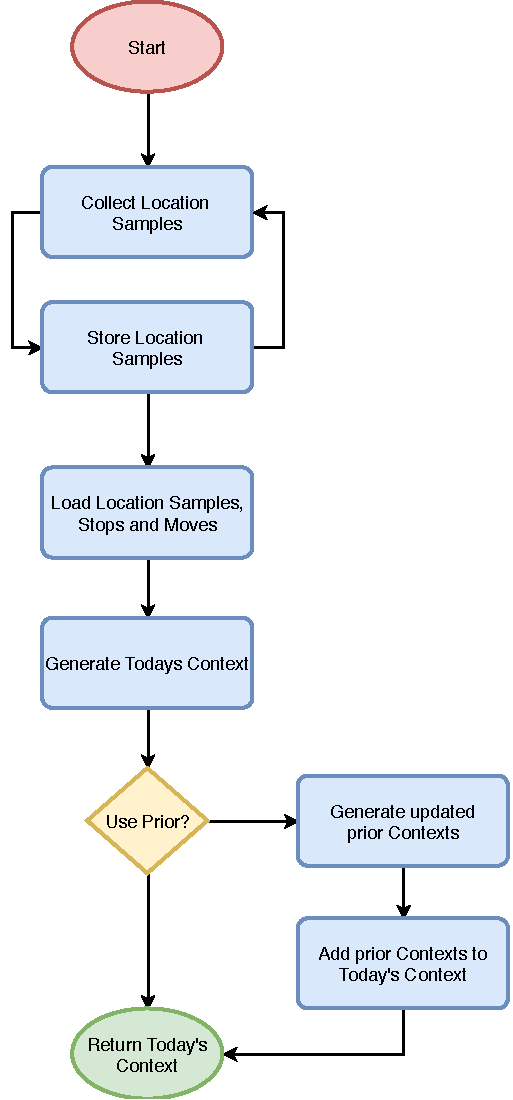
\includegraphics[width=0.5\textwidth]{images/diagrams/api-flowchart.pdf}
    \caption{The flowchart for computing mobility features using historical data}
    \label{fig:flowchart-features}
\end{figure}

\begin{itemize}
    \item Saving and loading of Location Samples on the device
    \item Computing intermediate features from Location Samples
    \item Saving and loading Stops and Moves on the device
    \item Computing the features
\end{itemize}

Saving and loading of Location Samples is necessary to not lose data. When an application tracks location data for a prolonged period, i.e. a whole day, it will risky to keep all the collected data in RAM since all data is lost if the app is killed by accident either by the OS or the user. For computing the Routine Index it was necessary to store historical data, to compare days. Intermediate features made this possible by bringing the storage requirements down significantly, compared to storing raw Location Samples on the device. A normal day of tracking could result in up to 18,000 Location Samples which is quite a lot of data considering the algorithms need up to 28 days of data. Besides, converting a dataset of raw Location Samples into Stops also made the computation for finding Places, and thereby many of the mobility features, much cheaper. Lastly, computing mobility features should be possible at any time, even if the day is incomplete. This has been taken care of by the definitions made in Chapter \ref{chapter:03} by redefining features such that they can be evaluated on incomplete days. 

The road from starting with a blank slate to computing mobility is depicted in the flowchart in Figure \ref{fig:flowchart-features}. First, the programmer needs to initialize data collection and save the collected samples with some frequency. Exactly how this is done is left the programmer. When feature computation is requested, the stored data including Location Samples, Stops, and Moves are loaded into memory. The Mobility Context for today is computed from this data, and afterward, it is checked whether or not prior contexts should be used. If so, then the historical Stops and Moves are used to generate these, and they are added to the Context of today. In any case, today's Context is returned to the method caller.


% \subsection{Storing and Loading}
% Since historical data is a major factor in computing the features, it was decided to include an easy way for the programmer to store and load Location Samples. To store objects they can be each serialized into one Large Object as defined by Fowler \cite{fowler-PEEA} [p. 272] i.e. a graph of composite objects. A serialized object, in contrast to an entity stored in the database, is already pre-assembled. In a database, this assembly happens via joins since the object is spread over multiple tables. This is analogous to how a set of LEGO comes in a box of individual pieces rather than already being pre-assembled. While traditional databases usually scale better than serialization they come with an initial overhead cost of time, from a development point of view. For this reason, serialization was chosen in favor of databases,  since the project was of a small scale and time was of the essence. Also, it is very easy to import serialized objects into other programming languages, such as Python for data analysis. 

% \subsection{Data Format}
% The data format used was JSON (JavaScript Object Notation) which is a very common, human-readable data format that uses key-value pairs to store data. A JSON object can be stored in a database, or it can be transformed into a string to be stored. It was chosen to simply transform JSON objects to a string and write them to a local file, rather than storing the information in a database on the phone. JSON supports a limited number of simple data types, such as strings, numbers, booleans, arrays, objects, and null values. This means that to translate a runtime object to JSON, all of the object's data must be serializable. Serialization, therefore, requires components that are to be serialized to be converted into some representation which is purely consisting of these simpler data types.

